%%%%%%%%%%%%%%%%%%%%%%%%%%%%%%%%%%%%%%%%%%%%%%%%%%%%%%%%%%%%%%%%%%%%%%%%%%%
%% This file is part of the book
%%
%% Algorithmic Graph Theory
%% http://code.google.com/p/graph-theory-algorithms-book/
%%
%% Copyright (C) 2009, 2010, 2011 Minh Van Nguyen <nguyenminh2@gmail.com>
%%
%% See the file COPYING for copying conditions.
%%%%%%%%%%%%%%%%%%%%%%%%%%%%%%%%%%%%%%%%%%%%%%%%%%%%%%%%%%%%%%%%%%%%%%%%%%%

\documentclass{article}

\usepackage{tikz}
\usetikzlibrary{external}
\usetikzlibrary{trees}
\tikzexternalize{Bernoulli-family-tree}

\begin{document}

\begin{figure}
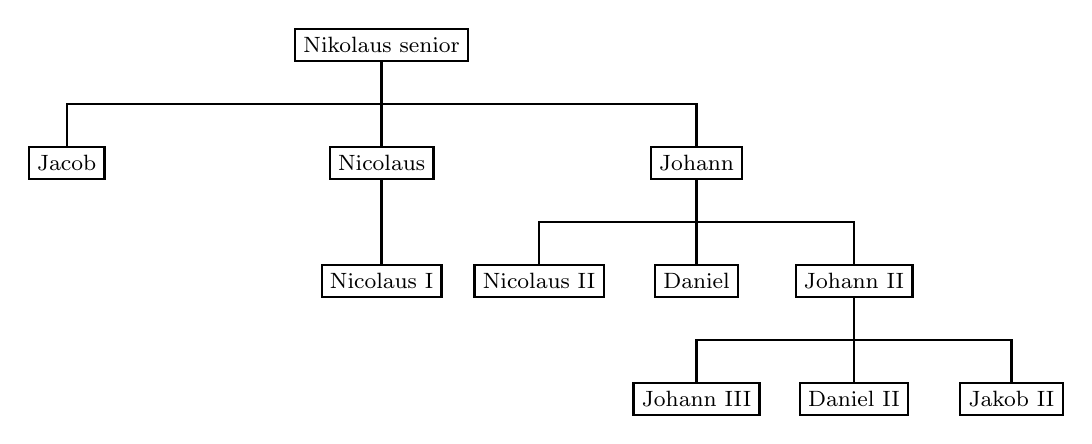
\begin{tikzpicture}
[-,thick,%
  every node/.style={shape=rectangle,inner sep=3pt,draw,thick}]
\footnotesize
\node {Nikolaus senior} [edge from parent fork down]
  [sibling distance=4cm]
  child {node {Jacob}}
  child {node {Nicolaus}
    child {node {Nicolaus I}}
  }
  child {node {Johann}
    [sibling distance=2cm]
    child {node {Nicolaus II}}
    child {node {Daniel}}
    child {node {Johann II}
      child {node {Johann III}}
      child {node {Daniel II}}
      child {node {Jakob II}}
    }
  };
\end{tikzpicture}
\end{figure}

\end{document}
